% This is LLNCS.DEM the demonstration file of
% the LaTeX macro package from Springer-Verlag
% for Lecture Notes in Computer Science,
% version 2.3 for LaTeX2e
%
\documentclass{llncs}
%
\usepackage{makeidx}  % allows for indexgeneration
\usepackage[utf8]{inputenc}
\usepackage[english]{babel}
\usepackage{indentfirst}
\usepackage{graphicx}
\usepackage{subfig}
%
\begin{document}

\mainmatter              % start of the contributions
%
\title{Text Mining Wikipedia\\to extract historical facts}
%
\titlerunning{Text Mining Wikipedia\\to extract historical facts}  % abbreviated title (for running head)
%                                     also used for the TOC unless
%                                     \toctitle is used
%
\author{João Valente\inst{1} \and João Gradim\inst{1}}
%
\authorrunning{João Valente, João Gradim}   % abbreviated author list (for running head)
%
%%%% list of authors for the TOC (use if author list has to be modified)
\tocauthor{João Valente, João Gradim}
%
\institute{Faculdade de Engenharia da Universidade do Porto,\\
Rua do Dr. Roberto Frias, s/n, Porto, Portugal}

\maketitle              % typeset the title of the contribution

\begin{abstract}
The abstract should summarize the contents of the paper
using at least 70 and at most 150 words. It will be set in 9-point
font size and be inset 1.0 cm from the right and left margins.
There will be two blank lines before and after the Abstract. \dots
\end{abstract}

\section{Problem}

\section{Objectives}

\begin{itemize}
	\item To provide an easily queryable database of historical events of major importance
	\item To allow users to use natural language to perform queries
	\item To be able to cross-reference historical events and link figures, places
	\item To be able to group events in categories to further refine search
\end{itemize}

\section{Motivation}

Younger population knows progressively less and less about history and human achievements. A simple interface would provide a means to an easy access to information and could boost interest in learning.\\

\section{State of the Art}

Text mining is the process of extracting high quality, useful data from text. This can be accomplished through semantical and phrasal structure analysis. The Stanford Parser is a probabilist parser that aims to produce the \textit{most likely} analysis of new sentences; although this can sometimes lead to some errors, the overall result is very satisfactory, producing acurate trees for almost every parsed sentence(s).\\

Text classification is a problem that aims to categorize documents or simple sentences in one or more categories, based on their contents. This can be achieved using either Support Vector Machines or a Naïve Bayes classifier. Unlike Support Vector Machines, which produce a \textit{binary classification}, i.e. either the text is in a certain category or isn't, a Naïve Bayes classifier allows for a number of arbitrary categories. A Naïve Bayes classifier can be trained using a set of pre-classified sentences in a \textit{supervised learning} setting, yielding very satisfactory results when classifying unknown sentences (about 80\%-90\% of correct results, depending on the size and quality of the training set).

\section{Text Extraction}

\section{Text classification}

\section{Natural Language Processing}

A parse tree containing the phrasal structure of a sentence can be obtained by using the \verb!LexicalizedParser! class present in the Stanford Parser. This tree can be used to derive (if present) either the location of the event and the people involved. Sections \ref{chp:people-extraction} and \ref{chp:local-extraction} show the tree structures used for the extraction of such informations.

\subsection{People Extraction}
\label{chp:people-extraction}

\begin{figure}[h]
	\centering
	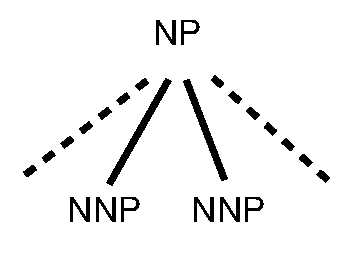
\includegraphics[width=40mm]{dia/people.eps}
	\caption{People extraction tree pattern}
	\label{fig:people-extraction}
\end{figure}

Figure \ref{fig:people-extraction} shows the subtree relating to singular proper nouns (NNP) nodes, from where people involved in the event can be extracted. As the phrasal structure does not allow for easy extraction of this information (this structure alone can not infer if the proper nouns refer to a country or a name or even a brand), only when an NP (noun phrase) node has at least two contiguous NNP child nodes is a name extracted.

\newpage
\subsection{Local extraction}
\label{chp:local-extraction}

\begin{figure}[h]
	\centering
	\subfloat[Location extraction tree pattern 1]{\label{fig:local_1}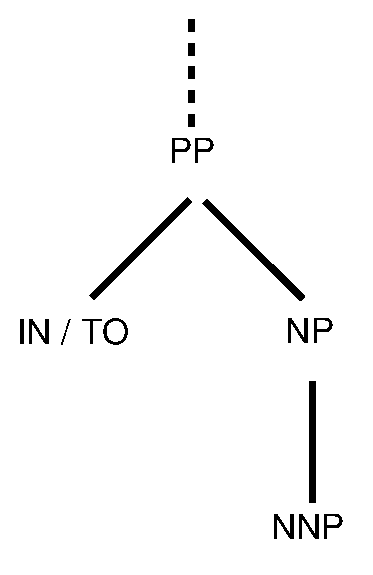
\includegraphics[width=0.3\textwidth]{dia/local_1.eps}}     
	\hspace{20mm}
	\subfloat[Location extraction tree pattern 2]{\label{fig:local_2}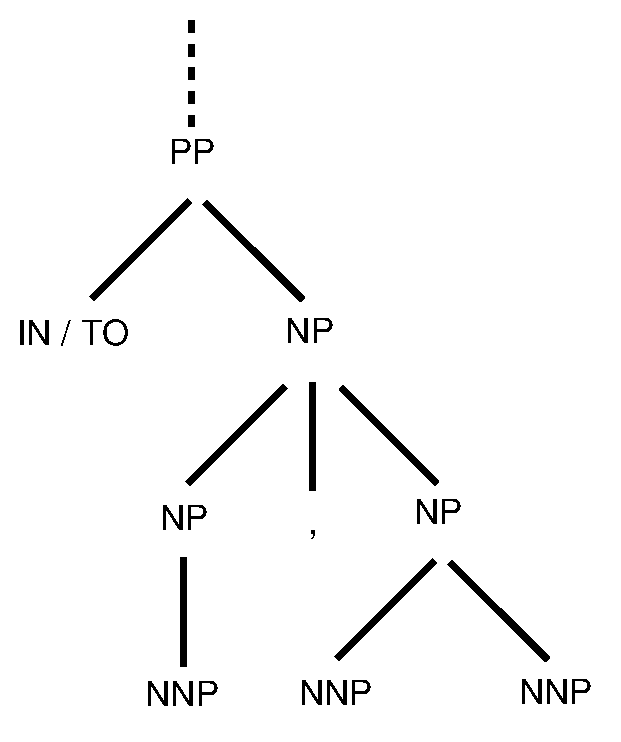
\includegraphics[width=0.4\textwidth]{dia/local_2.eps}}
	\caption{Subtrees for event location extraction}
	\label{fig:location-extraction}
\end{figure}

This kind of structure is present on most events parsed from Wikipedia and allows the retrieval of the phisical location of the occurence, mainly the country or a city in a determined country.

%
\section{Main implementation problems}

Wikipedia is an open knowledge base, relying mainly on user generated content. As such, it's difficult to ensure a proper and constant textual structure for information. Although the pages for the most recent centuries (aprox. 18th century) have a well defined an constant HTML strutcture that allows for reliable information retrieval, there are many years that don't follow this structure, leading to specific parsing cases.\\
\ \\
This openness lead to another problem: an HTML structure not suited for easy parsing. A series of workarounds had to be implemented to successfuly extract useful information.

\newpage
%
% ---- Bibliography ----
%
\begin{thebibliography}{}
%
\bibitem[1990]{santorini}
Santorini, B. :
Part-of-Speech Tagging Guidelines for the
Penn Treebank Project (3rd Revision, 2nd Printing).
(July 1990)

\bibitem[1995]{bies}
Bies, A., Ferguson, M., Katz, K., MacIntyre, R. :
Bracketing Guidelines for Treebank II
Penn Treebank Project
(June 1995)

\end{thebibliography}
\clearpage
\addtocmark[2]{Author Index} % additional numbered TOC entry
\renewcommand{\indexname}{Author Index}
\printindex
\clearpage
\addtocmark[2]{Subject Index} % additional numbered TOC entry
\markboth{Subject Index}{Subject Index}
\renewcommand{\indexname}{Subject Index}
\input{subjidx.ind}
\end{document}
